% Chapter 1

\chapter{Alevin 2} % Main chapter title

\label{alevin2} % For referencing the chapter elsewhere, use \ref{Chapter1} 

%----------------------------------------------------------------------------------------

\section{Background}

RNA-seq quantification has been shown as an important tool to explore the genome-wide
quantification of gene expressions for both bulk and \singlecell RNA-seq experiments.
\dscrnaseq experiments have been especially useful, as with the advancement in droplet-based 
sequencing technologies ~\citep{dropseq, indrop, tenx}, it can generate data with high 
quantitative accuracy, sensitivity, and throughput. In ~\Cref{alevin}, we discussed a 
principled framework for generating cell-wise gene-expression estimates given the read sequences
from a \dscrnaseq experiment. We showed how discarding gene-multi mapping reads, typically done 
by all the existing \dscrnaseq quantification pipelines, can lead to biased expression estimates. 
Specifically, after the UMI resolution phase, we assign the ambiguous reads with more than 1 gene label to
genes based on an expectation-maximization (EM) algorithm. Although the framework works well in most of the cases, 
in situations where there is no unique read evidence to confidently disambiguate the read assignment
among genes, which we refer to as tier-3 estimates, the likelihood estimator uniformly divides the reads 
across the genes in the equivalence class label. In this study, we propose the idea of information sharing across closely 
related cells using Bayesian priors for specifically improving these tier-3 estimates. Since we expect cells in an experiment
to fall into categories of specific cell-types, and cells within a cell-type to have similar expression patterns, we propose that
sharing information across neighboring cells in the expression space will improve quantification 
estimates of the individual cells. We show that our idea of information sharing using Bayesian 
priors to improve quantification can be successfully applied to a \dscrnaseq experiment and results in higher accuracy estimates.

\section{Material and Methods}
\label{sec:alv2_methods}

\subsection{Variational Bayesian \dscrnaseq quantification}
Similar to \salmon 's ~\citep{salmon} collapsed Variational Bayesian (VB) optimization 
objective, we aim to quantify the expression, given a set of known genes $\mathcal{G}$ and a set
of gene-level equivalence classes with their UMI counts, generated post UMI deduplication using \alevin 's 
framework, as $\mathcal{E}$. Originally, \alevin takes a maximum-likelihood based approach to 
optimize the gene-level ambiguous read assignment objective. However, it cannot utilize the 
confidence from neighboring cells. Since a high level of sparsity is an inherent property of a \dscrnaseq
experiment and due to the random process of capturing RNA molecules, in expectation, molecule 
sampling noise wouldn't be uniform across all cells. We expect that sharing confidence in 
the expression estimates across cells can be particularly effective in improving cell-level expression. 

\salmon is a bulk RNA-seq quantification tool that uses Bayesian priors to improve the 
quantification estimates by its online learning phase. We use the relaxed version of the algorithm 
to improve the estimates of \alevin. Specifically, if we define gene-UMI count 
assignment matrix as $\mathcal{Z}$, where based on $\mathcal{E}$, $z_{ij}=1$ if UMI $j$ is derived from 
gene $i$. We also define the probability of generating a molecule from a particular gene as $\rho$ (analogous to 
nucleotide fraction in \salmon model); we can write the probability of observing a set of deduplicated 
UMIs $\mathcal{U}$ as follows:

\begin{equation}
    \Pr\{\mathcal{U} | \mathcal{Z},\mathcal{G}\} = 
    \prod_{j=1}^{N}\sum_{i=1}^{M}\Pr\{ g_i | \rho \} \cdot \Pr\{ u_j | g_j, z_{i,j} = 1 \}
\end{equation}
 
 where $|\mathcal{U}| = N$ is the number of total molecules in the experiment (i.e. the number of 
 deduplicated UMIs ) and $|\mathcal{G}| = M$ is the number of total genes.
 
In this study we take the Bayesian approach for gene-expression estimation i.e. instead of 
seeking the maximum-likelihood estimates we infer the posterior distribution of $\rho$. 
This posterior distribution can be defined as:

\begin{equation}
    \Pr \{ \rho | \mathcal{U}, \mathcal{G} \} 
    \propto \sum_{\mathcal{Z}} \Pr\{ \mathcal{U} | \mathcal{G}, \mathcal{Z} \}
    \cdot \Pr\{ \mathcal{Z} | \rho \} \cdot \Pr\{ \rho \}
\end{equation}

where both $\Pr\{ \mathcal{U} | \mathcal{G}, \mathcal{Z} \}$ and $\Pr\{ \mathcal{Z} | \rho \}$ are 
data-dependent observables and can be estimated as defined in ~\citet{salmon}. The novelty of our method
comes with setting the prior term $\Pr\{ \rho \}$ specifically for \dscrnaseq data. We perform
intra-sample anchoring using Seurat3 (details in ~\Cref{subsec:anchor}) and use the gene expression
estimates from the nearest cells (with anchoring score >0.5) to generate cell-specific prior.

\subsection{Cellular Barcode Anchoring}
\label{subsec:anchor}
In~\Cref{alevin} we defined tier 3 estimates as specifically the estimates which have reads assigned 
to gene ambiguous labels and that don't have any uniquely assignable read evidence in their equivalence 
class network. To disambiguate the gene assignment, we use 
information from cells with similar global expression profile within the sample. To find similar cells for sharing 
the confidence in their gene expression estimates we use Seurat's~\citep{seurat3} cellular
barcode anchoring scheme. In Seurat,~\citet{seurat3} proposed an anchoring scheme in which they 
defined a framework to connect two experiments based on the similarity in their cell's gene expression 
pattern. They first find the nearest neighbor using l2 distance of both inter and intra datasets to generate 
four distance matrices. Later, they look for cells which are neighbors to each other in both 
directions to define anchors connecting two cells with similar looking expression patterns 
across different \singlecell datasets. We use the same anchoring algorithm to connect two similar 
cells and define the priors in the Bayesian estimation of gene expression.

The anchoring process can sometimes generate multi-mapping in both directions. To compensate for this we take 
average of all the neighboring cells which have been chosen as the anchor to define the prior. In a typical 4000 \singlecell 
experiment, we run \alevin and repeat the Seurat3 anchoring approach $30$ times, randomly dividing 
the cells into two equal sets and mapping one set onto the other. We use anchors with score $>0.5$ as a potential list 
of neighboring cells to define the priors. This prior is then used to optimize the quantification estimates of genes 
with multi-mapping reads in the \alevin pipeline. As a proof-of-concept, we use the prior with only tier 3 estimates, 
while keeping uniform prior for both tier 1 and tier 2 estimates.

\section{Results}
One fundamental property of \dscrnaseq experiments is that molecules are randomly captured across cells 
and, although some cells might randomly sample the read sequence from the ambiguous region 
(or not sample at all), in expectation, similar cells in a group can potentially have different 
confidence in their gene estimates. 

\begin{figure}[!htb]
    \centering
    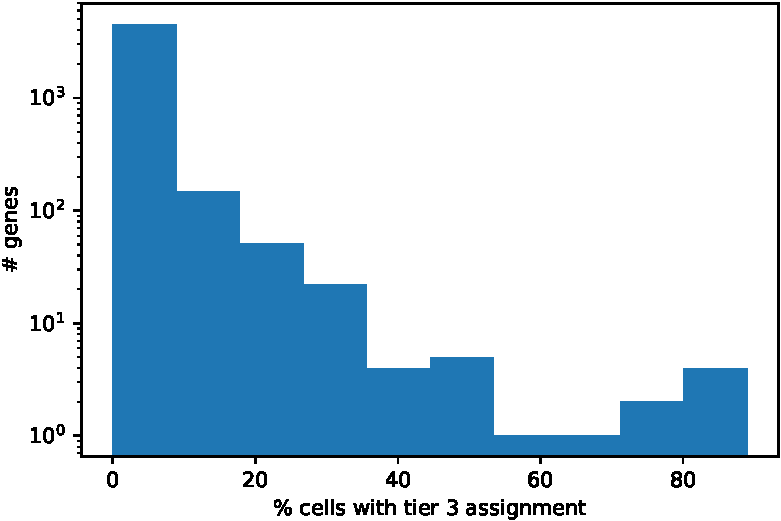
\includegraphics[height=3in]{alevin2/t3_assign.pdf}
    \caption{ The distribution of the number of genes with the fraction of cells that have tier 3
    assignment.}
    \label{fig:alv2_t3}
\end{figure}

In~\Cref{alevin}, we categorize the confidence in the generated gene counts estimates using tiers. 
Even though we show that the \alevin generated quantification estimates are accurate, the confidence 
in tier 3 assigned estimates is low and often a source of mis-estimation. In~\Cref{fig:alv2_t3} we show the 
distribution of genes with the fraction of cells that have tier 3 estimates. This motivates our idea that to improve 
the expression estimates of tier 3 genes, we can utilize the independent sampling of neighboring cells and share 
information across them to improve gene-level estimates (details in~\Cref{sec:alv2_methods}).

\subsection{Variational Bayesian Estimation with Informative Priors Improves \dscrnaseq quantification}
Over the years, with the advancement in \singlecell technologies, various \singlecell quantification 
pipelines have been proposed. However, non-availability of validation datasets and/or criteria for 
comparing gene-expression estimates generated by the various pipelines has been lacking. 

\subsection{Comparing quantification methods on simulated data}
\label{subsec:alv2_sims}

To compare gene estimates, we had previously proposed an empirical \dscrnaseq data simulation tool, 
Minnow~\citep{sarkar2019minnow}. Minnow models various features involved in the generation of the \dscrnaseq data, 
like PCR amplification and sequencing errors to generate fastq file with the reads and the expected true cell 
by gene counts. We used minnow to simulate a \dscrnaseq experiment with 4340 human PBMC cells with $\sim$
20 Million UMIs and compared the quantification estimates generated by various methods. We found that, 
in the simulated data, more than 66\% of the false discoveries made by \alevin are in the tier 3 estimates 
and due to the inherent problem of sparsity in \dscrnaseq data, we expect a similar pattern of tier 3 genes in 
the real data as well.

We validated our prior enhanced VBEM approach on simulated data using the minnow generated data (details in~\Cref{subsec:alv2_sims}). 
We first used EM based \alevin on the simulated data to generate quantification
estimates on 4340 cells. We used Seurat's anchoring scheme to self anchor the estimates and generate the
prior. Using the learned prior we re-quantified the simulated dataset with our VBEM based approach to generate 
the new estimates. In ~\Cref{fig:alv2_sim_val}, we compare the cell-wise correlation of both EM and  VBEM 
based approaches to the minnow generated ground truth and observe a higher correlation with VBEM generated
gene expression estimates.

  \begin{figure}[!htb]
      \centering
    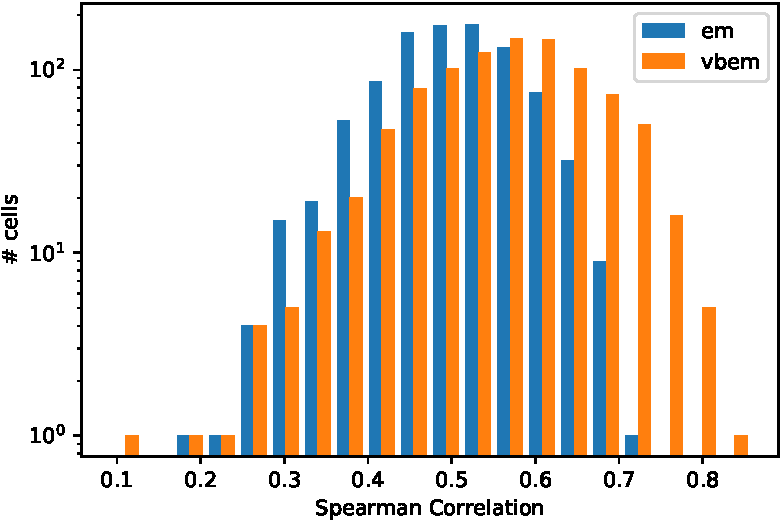
\includegraphics[height=3in]{alevin2/sim_corr.pdf}
    \caption{ Comparison of the cell-wise spearman correlation of EM based \alevin with VBEM based
    prior enhanced \alevin on simulated experiment}
    \label{fig:alv2_sim_val}
  \end{figure}

\subsection{Knock Out Experiment on Real Data}
\label{subsec:alv2_real}
We validated that the Variational Bayesian estimation of \alevin is more accurate on real data using the
following knock out (KO) experiment. \Alevin 's pipeline for \dscrnaseq quantification has multiple 
phases. After the initial phases of whitelisting and read-mapping, \alevin generates an interim 
file format, called bfh, which contains the transcript equivalence classes along with their Cellular
Barcode and UMI count. A major fraction of tier 1 estimates come from unique transcript equivalence
classes. In our KO experiment, we knocked out all unique transcript equivalence classes, with
the expectation that the KO bfh will migrate some of the tier 1 and tier 2 estimates to tier 3, as they have
may lose the unique information which made them high confidence tiers (tier 1 and tier 2) to start with. 

  \begin{figure}[!htb]
      \centering
    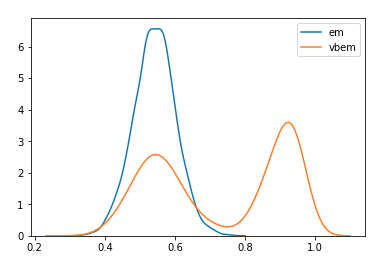
\includegraphics[height=3in]{alevin2/migration.png}
    \caption{ Comparison of the cell-wise spearman correlation of EM based \alevin with  VBEM  based
    prior enhanced \alevin on real data KO experiment}
    \label{fig:alv2_real_val}
  \end{figure}

We took the quantification estimates from the pbmc\_4k experiment with 4340 cells and randomly divided it into
two parts of 2170 cells each, we call 2ka and 2kb experiment. We performed the KO experiment on
2ka cells and generated \alevin EM estimates using KO bfh. Later, we anchored KO 2ka estimates 
with full 2kb estimates and learned informative priors for KO 2ka estimates to re-quantify using \alevin  VBEM 
approach. In ~\Cref{fig:alv2_real_val}, we show the cell-wise correlation of KO 2ka experiment (as em) and prior
enhanced version of \alevin (as  VBEM ). Since the anchoring scheme can't always find high confidence anchors for 
all cells, we see a bimodal distribution with VBEM approach which signifies the first mode (overlapping 
with em) are cells with no informative prior while the second mode (with improved correlation)
signifies cells where information can be discovered.

\section{Conclusion}
We proposed a Bayesian framework that extends \alevin 's maximum likelihood-based 
quantification procedure. We explore different techniques of generating priors and show that our 
information-sharing framework consistently improves the tier 3 \dscrnaseq quantification estimates and 
is especially useful for highly ambiguous estimates where there is no intracellular unique information to 
efficiently quantify. We plan to extend the framework to incorporate priors from new 
technologies, For example, spatial data can be useful for setting the prior in the proposed 
\alevin framework.  We think this framework has the potential to open a new direction of enabling 
multi-modal information sharing to improve the quantification of the data.